%%%%%%%%%%%%%%%%%%%%%%%%%%%%%%%%%%%%%%%%%
% implementazione_del_sistema_rmi.tex v1.0
%
% Relazione per il progetto PuzzleSolver (Parte 3)
% Autore: Giacomo Cusinato
% Materia: Programmazione Concorrente e Distribuita
%
%%%%%%%%%%%%%%%%%%%%%%%%%%%%%%%%%%%%%%%%%

\section{Implementazione del sistema RMI}

\begin{figure}[htbp]
    \centering
    \centerline{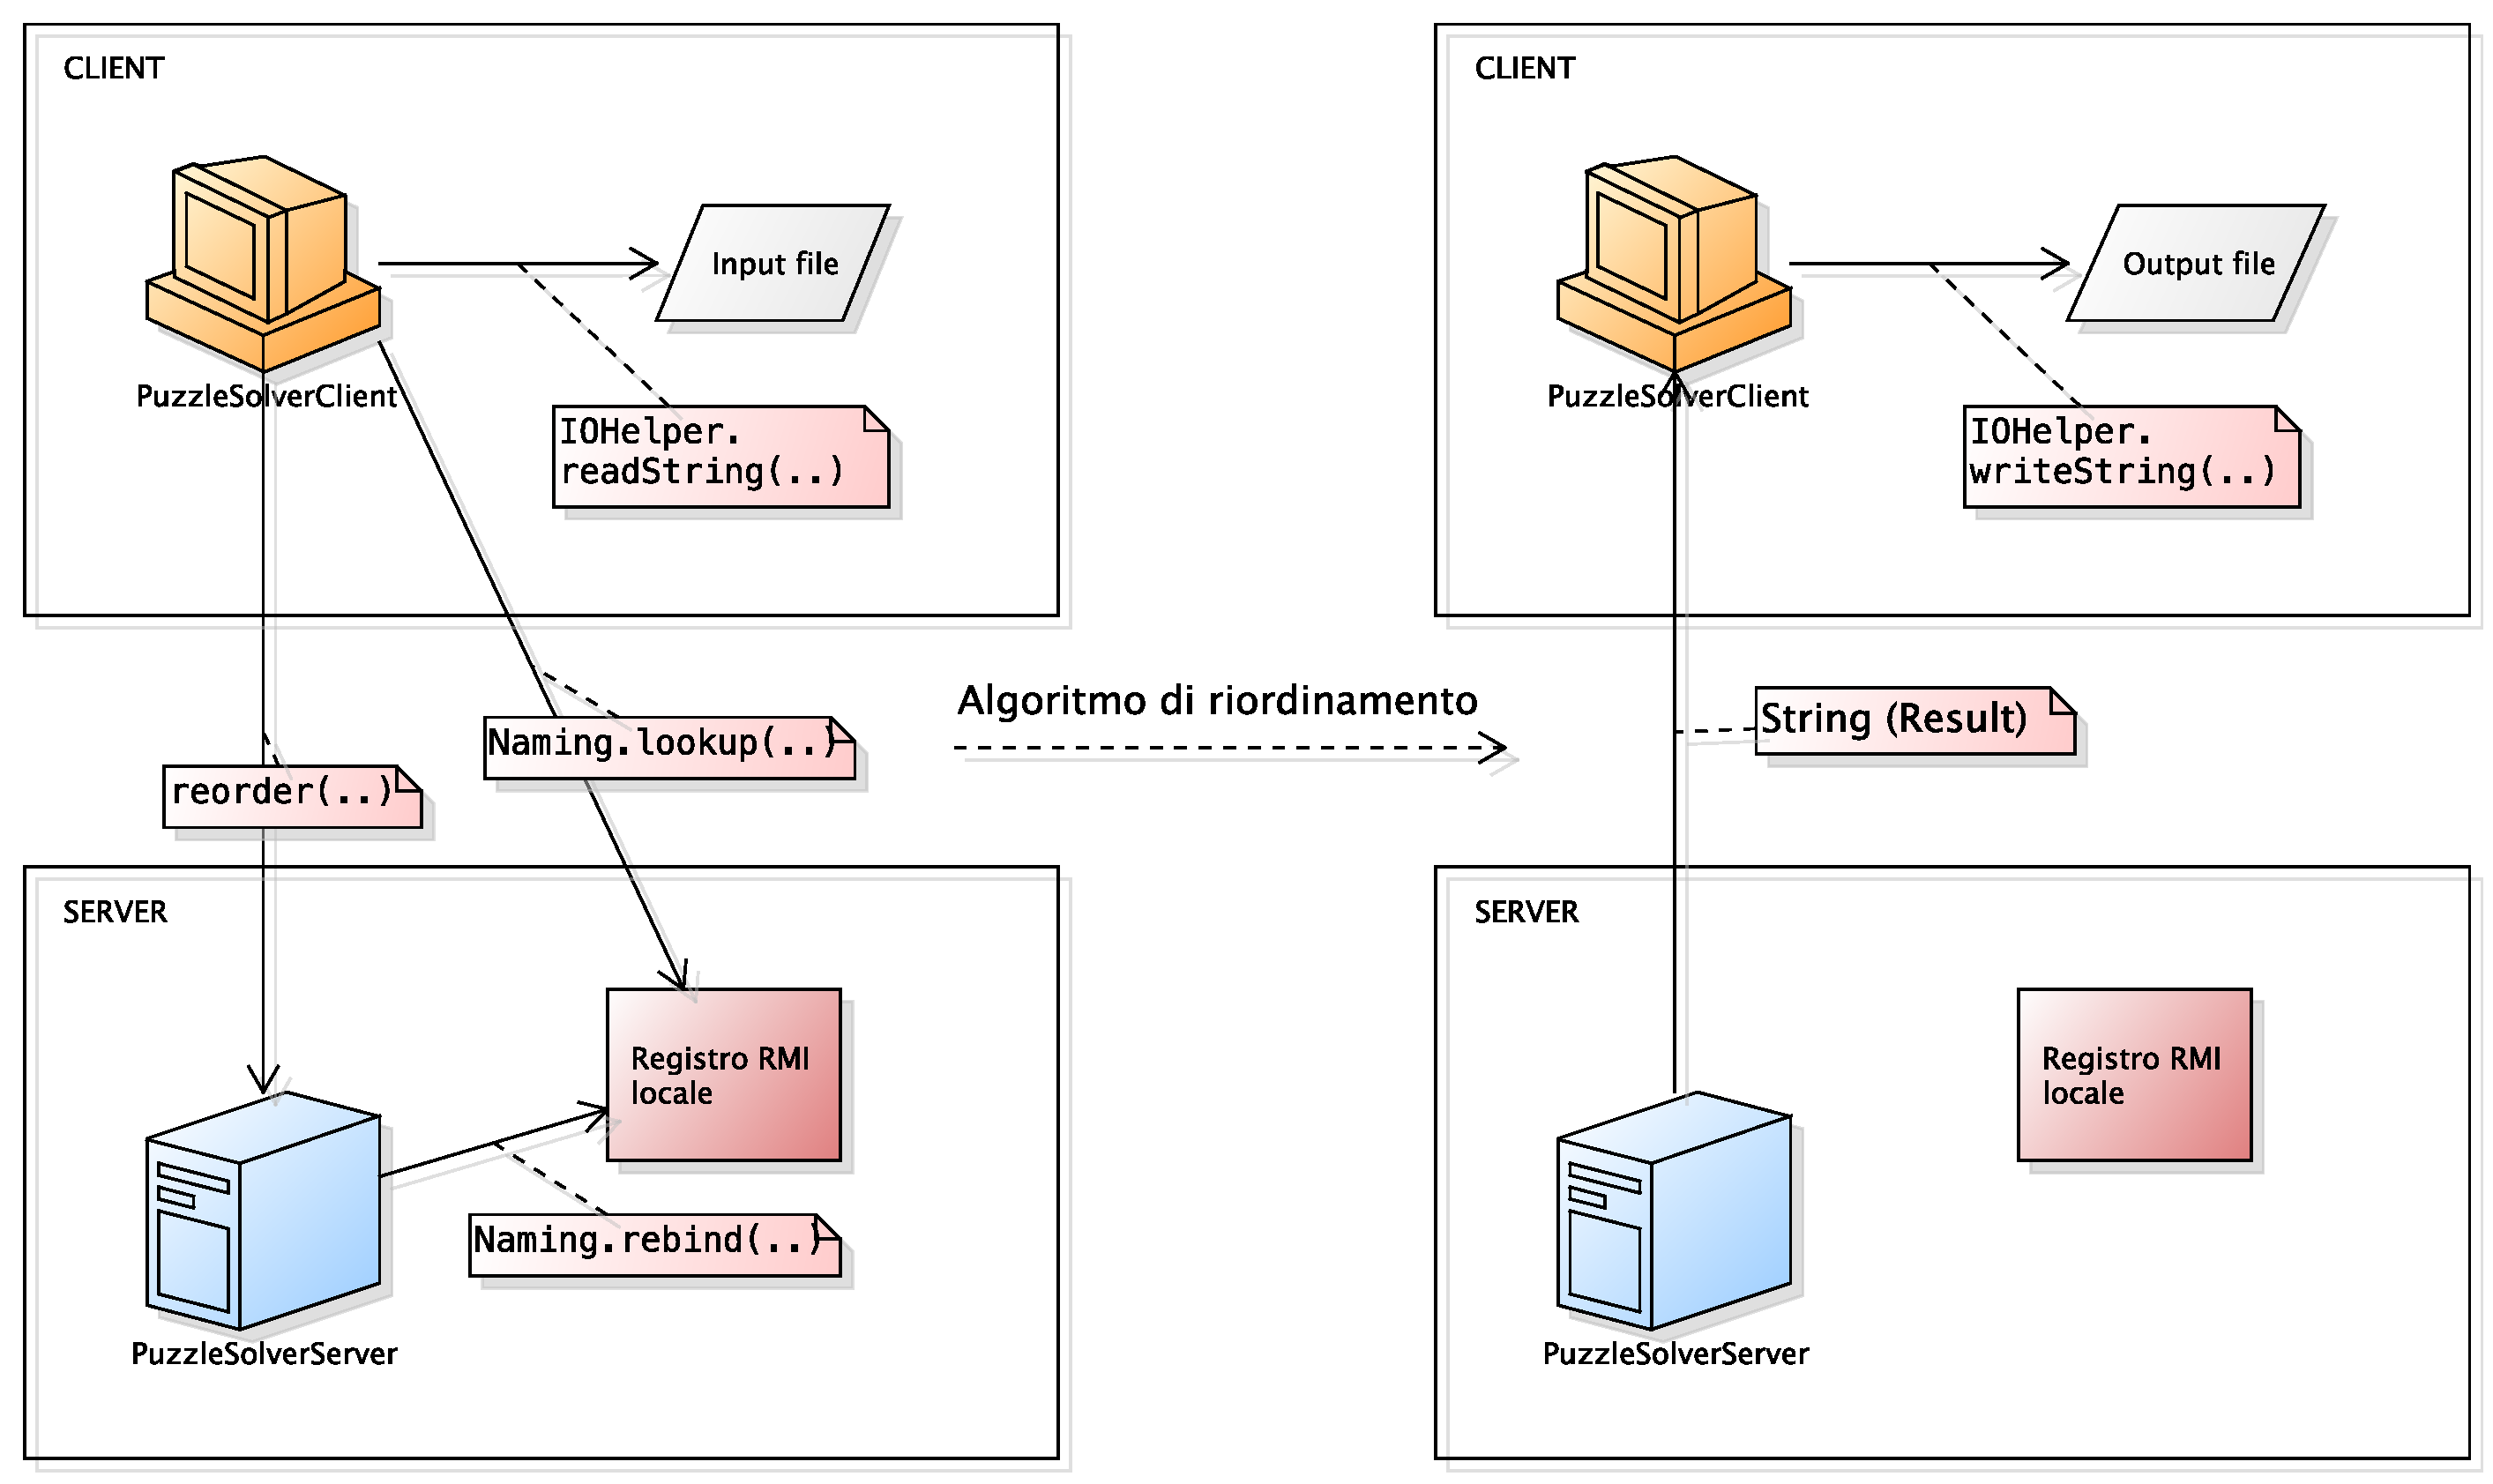
\includegraphics[scale=0.4]{./images/rmi.pdf}}
    \caption{Vista generale implementazione RMI in PuzzleSolver}
\end{figure}

\subsection{L'intefaccia ISolver}

L'interfaccia \texttt{ISolver} estende l'interfaccia \texttt{Remote} che fa da semplice marcatore di tipo
per l'oggetto remoto. \texttt{ISolver} contiene solamente la definizione del metodo remoto \texttt{reoder(String inputPath)},
che sarà implementato dalla classe \texttt{PuzzleSolverServer} con l'algoritmo di risoluzione. Tale metodo, può provocare
un'eccezione di tipo \texttt{RemoteException} a causa di eventiuali problemi di connessione o comunicazione col server.
L'interfaccia è presente sia nel modulo server che nel modulo client, quest'ultimo, infatti, necessita esclusivamente della
definizione del meteodo remoto da invocare visto che non sarà la JVM che risiede nel client ad eseguirlo.


\subsection{La classe PuzzleSolverServer}

L'instanza di questa classe rappresenta l'oggetto remoto il cui riferimento viene reso disponibile al client.
Il \texttt{main} della classe, infatti, crea un oggetto di tipo \texttt{PuzzleSolverServer} e tramite il medoto statico
\texttt{rebind(String uri, Remote obj)} della classe \texttt{Naming} registra l'instanza dell'oggetto creato nel
registro RMI locale. La stringa \texttt{uri}, contenente il nome del server e l'identificativo associato all'oggetto, sarà
utilizzata anche dal client per ottenere il riferimento a tale oggetto.
La classe \texttt{PuzzleSolverServer} espone il metodo remoto \texttt{reorder(String inputPath)} che può essere invocato
da una JVM remota ed esegue l'algoritmo di risoluzione del puzzle. Il metodo è stato dichiarato tramite la keyword
\texttt{synchronized} in modo che il server possa gestire più client in attesa mentre esegue l'algoritmo per il client attivo.
Il metodo \texttt{reset()}, inoltre, assicura che il valore di tutti i campi dati venga risportato a quello originale per
il corretto funzionamento del metodo \texttt{reoder(String inputPath)} invocato dal client sucessivo.


\subsection{La classe PuzzleSolverClient}

La classe \texttt{PuzzleSolverClient}, una volta letto il contenuto dle file di input, si occupa di ottenere un riferimento
all'oggetto instanziato sul server. Questo è possibile tramite il metodo statico \texttt{lookup(String uri)} della classe
\texttt{Naming} che interroga il registro RMI remoto e ottiene il riferimento all'oggetto grazie all'\texttt{uri} identificativo
associato. Inoltre il client, che contiene a sua volta la definizione dell'intefaccia \texttt{ISolver}, può ottenere il
riferimento remoto effettuando un downcast proprio ad un oggetto di tipo \texttt{ISolver}, su cui è possibile invocare il metodo
remoto \texttt{reorder(String inputPath)}.
